
\subsection{Velocity estimation}
When evaluating the experimental data from the first lab session, it became clear that there were some problems with the positioning camera system. During a experiment, due to a combination of calibration inaccuracies and motion, the infrared reflector orbs on the ship can cause "reflection shadow", thus leading to a small jump in position. This phenomenon is shown in Fig. \ref{fig:measurements_spring}. While the might only be 2 cm in magnitude, it occurs in a single time sample of 10 milliseconds, which results in a sudden velocity change of 2 m/s, which is not only a physically unreachable velocity for the ship, but also beyond the feasible acceleration. Since the estimated velocity is fed back into the control system, it causes the controller to try to compensate for the non-physical behavior, leading to a noisy control signal and also higher wear on the actuators.   


\begin{figure}[!h]
    \centering
    \makebox[\textwidth][c]{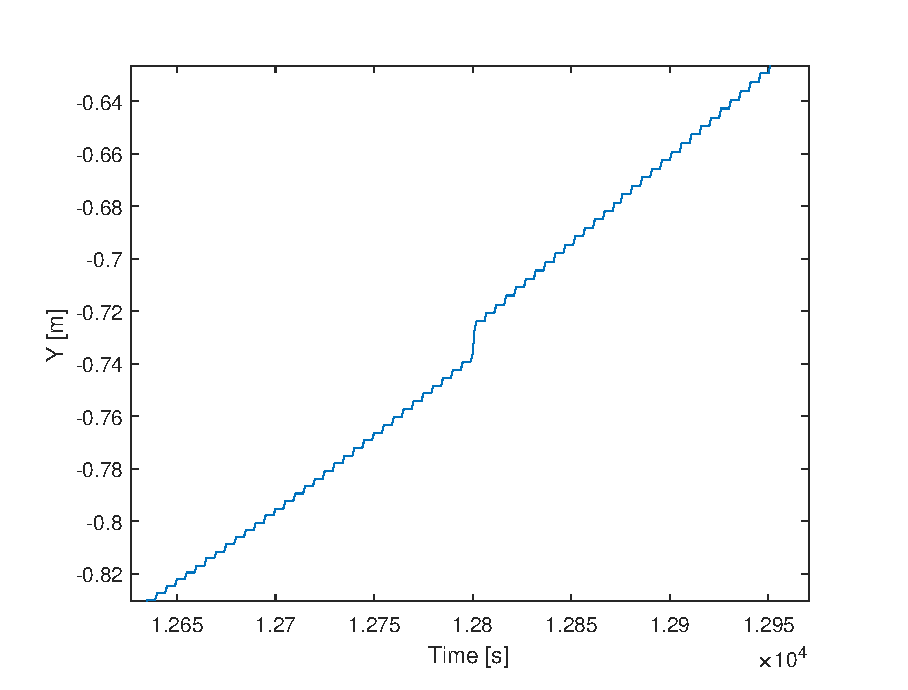
\includegraphics[width=0.7\textwidth]{plots/spring_phenomenon.eps}}
    \caption{ Jump-phenomenon in pose measurement}\label{fig:measurements_spring}
\end{figure}

The correct for this behavior, some changes to the estimator are done; 
The velocity estimator previously implemented in CSAD for the lab is a applied derivative filter. Augmenting this filter to compensate for the "spring"-effect, maximal values for CSAD feasible acceleration were set as follows: 
\begin{align}
    a_{surge}^{MAX} &= \pm 0.13 m/s^2 \\
    a_{sway}^{MAX} &= \pm 0.0267 m/s^2 \\
    a_{yaw}^{MAX} &= 0.0052 rad/s^2
\end{align}

These maximal values are determined through velocity test in the MC-lab basin, using CSAD on maximum thrust in each degree-of-freedom. Since the control system runs at 100Hz, these limit parameters are then scaled by 100 to get allowed change-per-sample, and then implemented in block form in the derivative filter. Only minor tuning is then needed to achieve optimal cutting of impulse transients in the estimated velocity signal. The final limit values are displayed in Table \ref{acc_limits_CSAD}. It should be noted that these are vessel-specific, and should be adjusted in the event of a new actuator setup, or if using the control system on another vessel. 

\begin{figure}[!h]
    \centering
    \makebox[\textwidth][c]{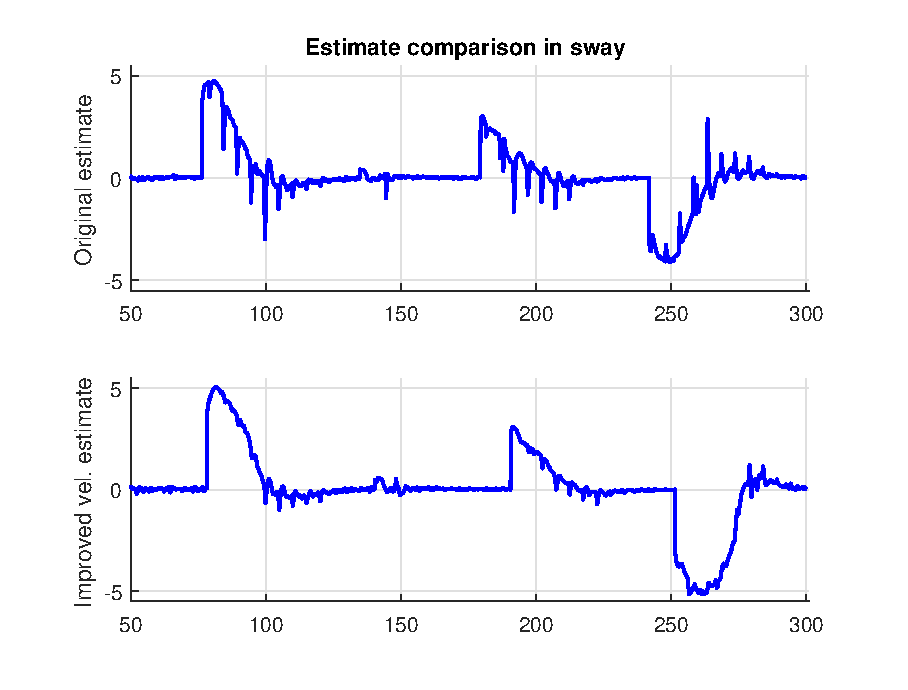
\includegraphics[width=0.85\textwidth]{plots/estimate_comparison.eps}}
    \caption{ Comparison of control input in sway with new velocity estimator}\label{fig:est_comparison}
\end{figure}

The effects of the estimator changes is illustrated in Fig. \ref{fig:est_comparison}. The figure shows the commanded input in sway for a 4-corner test using the the original and the improved velocity estimator. Both runs are done using the $\mathcal{L}_1$ cascade controller with the same controller and parameter gains. The experiments are done 10 minutes apart, giving identical water conditions in the MC-lab basin. While using the new estimator further might not affect the overall tracking accuracy of the controller significantly, it is beneficial in reducing actuator wear and tear, and can reduce power consumption, since the controller will not try to compensate for non-physical behavior. This is especially useful for the $\mathcal{L}_1$ cascade controller, due to its relatively high-gain adaptation, which leads to significant jerk in the actuator system. 

\begin{table}[!h]
\centering 
\begin{tabular}{| p{2cm} | p{2cm} |}
\hline
\textbf{DOF}& \textbf{Value}    \\ \hline\hline
$surge$ & $0.0011$   \\ \hline
$sway$ & $0.000454$  \\ \hline
$yaw$ & $0.00071$  \\ \hline
\end{tabular}
\caption{Acceleration limits per sample in velocity estimator}
\label{acc_limits_CSAD}
\end{table}

As previously discussed, the velocity estimator implemented in the lab prior has some design weaknesses. By design weaknesses, it is meant how it handles errors occurring in the camera-system, which cannot simply be corrected without extensive reconfiguration of the lab setup, only compensated for. Among these errors is the "spring-phenomenon", which in this new estimator design is handled by setting maximum values for the acceleration in each degree of freedom, per time sample. This corrects a lot of the spikes in the estimated velocity signal, thus leading to a smoother control signal, as seen in Fig 4.11. \\

Furthermore, to make the estimator more fault-tolerant, it is necessary to address the issue of a lost position signal. At some points, the Qualisys camera system will simply loose the view of the ship. To avoid giving a measurement of the basin origin, at $[0 0 0]^T$, which might lead to uncontrolled acceleration of the ship, the firmware of the system will simply give the last measured position in a loop until the ship is detected again, usually within a few samples. However, this approach will cause some unwanted effects. An example of the lost signal can be seen in Fig.\ref{fig:signal_freeze}. The estimated pose follows the measurement, since it is updated using the measurement signal. 

\begin{figure}[!h]
\centering
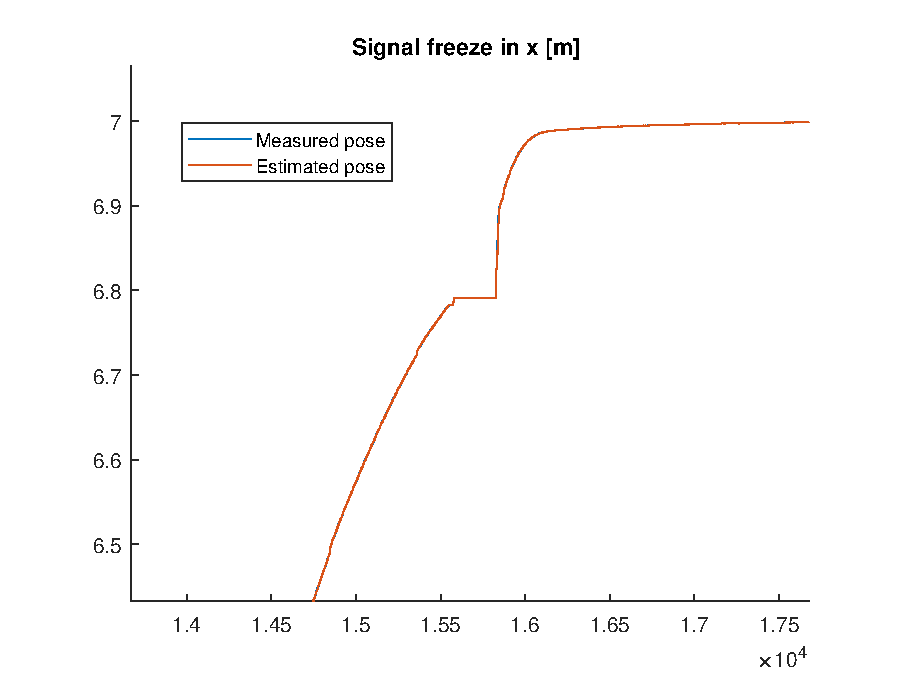
\includegraphics[width=0.9\textwidth]{plots/signal_freeze.eps}
\caption{"Frozen" measurement signal}
\label{fig:signal_freeze}
\end{figure}

In Fig. \ref{fig:signal_freeze}, as one can see, the pose measurement is still for around 250 samples, or 2,5 seconds, and while the control system assumes the ship is at a constant position, it is in the middle of a motion, and has a surge speed. When the camera system then again detects the ship, the pose is changed, and the estimate jumps to the new position, leading to a corresponding, sudden change in the velocity estimate, as seen in Fig. \ref{fig:surge_spike}. It is strongly desirable to avoid the velocity spikes, in addition to having a reliable estimate, to avoid false motions and thus noise in the control input. 

\begin{figure}[!h]
\centering
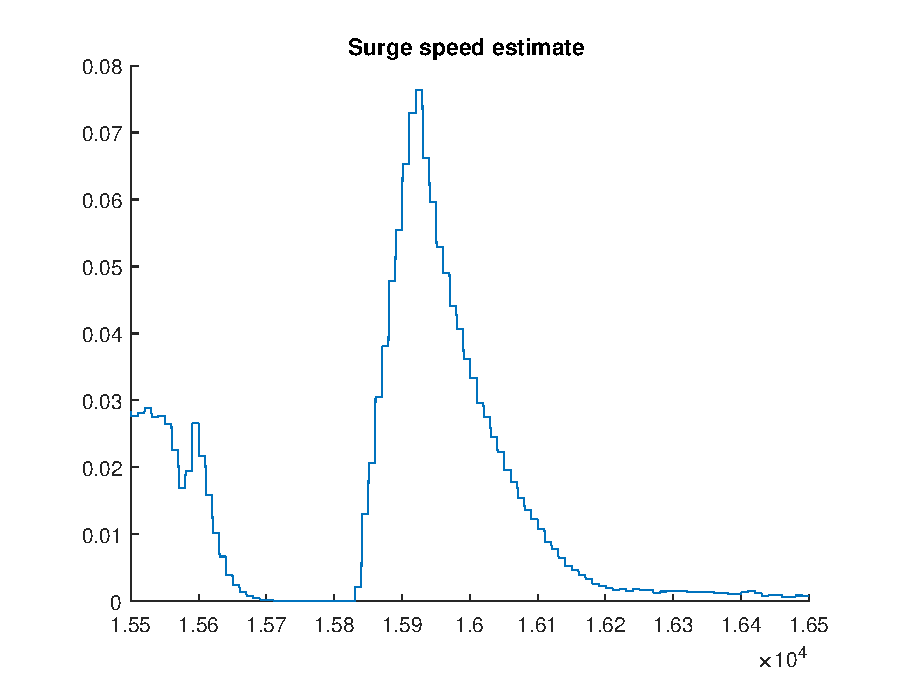
\includegraphics[width=0.9\textwidth]{plots/surge_spike.eps}
\caption{Sudden surge after recovering position measurement}
\label{fig:surge_spike}
\end{figure}

To ensure that the velocity estimator fault-tolerant to the phenomenons mentioned, and also more robust operation, a revision is proposed:\\ The estimator will have 3 states of operation; Normal operation, frozen measurement signal and rediscovered measurement signal. A subsystem is written in the control implementation, which compares each new sample to the previous down to the 8th decimal. The Qualisys system runs at 20Hz, while the control system runs at 100Hz, which means that every 5 consecutive samples from the camera system will be identical. If, however, the following sample is identical to the previous 5, at $10^8$ decimal precision in all DOF, the signal is assumed to have been lost. A Boolean "measurement frozen" signal is then sent to the estimator, which switches state. To avoid detecting false positives, the threshold for a lost signal is set to 7 consecutive identical measurement samples. 



The velocity estimator is written as a derivative filter using the pose measurements as input. For normal operation, this is implemented as such:
\begin{align}
    \boldsymbol{\eta}_{filtered(n)} &= a*\boldsymbol{\eta}_{measured(n)} + (1-a)*\boldsymbol{\eta}_{filtered(n-1)} \\
    \boldsymbol{\Dot{\eta}} &= \frac{\boldsymbol{\eta}_{filtered(n)}-\boldsymbol{\eta}_{filtered(n-1)}}{h} \\
    \boldsymbol{\Dot{\eta}}_{filtered(n)} &= b*\boldsymbol{\Dot{\eta}}_{measured} + (1-b)*\boldsymbol{\Dot{\eta}}_{filtered(n-1)}\\
    \boldsymbol{\hat{\nu}} &= \boldsymbol{R}^T(\psi)*\boldsymbol{\Dot{\eta}}_{filtered(n)},
\end{align}\label{eq:vel_estimator}
where h is the sample time in the control system, 0.01 second, and $a,b \in {\rm I\!R}$ are the cutoff-parameters for the filter. When the estimator detects a lost signal, it switches state and keeps the last recorded $\hat{\nu}$ to estimate the position until the camera system again detects the ship. While the signal is lost, the estimator will run as:

\begin{align}
    \boldsymbol{\hat{\eta}} &= \int \boldsymbol{R}(\hat{\psi})\boldsymbol{\hat{\nu}}\\
    \boldsymbol{\hat{\eta}}_{(0)} &= \boldsymbol{\hat{\eta}}_{(n-1)}
\end{align}

Then, when the measurement signal is recovered, it switches back to \ref{eq:vel_estimator}, and then initialized by:

\begin{align}
    \boldsymbol{\eta}_{filtered(n-1)} &= \boldsymbol{\hat{\eta}}_{(n-1)} \\
    \boldsymbol{\Dot{\eta}}_{filtered(n-1)} &= \boldsymbol{\hat{\nu}}_{(n-1)}
\end{align}
The block diagram for the re-written velocity estimator as implemented on CSAD can be seen in Fig. \ref{fig:estimator_blockdiagram}.

\begin{figure}
    \centering
    \begin{tikzpicture}
    \draw (-9,0.2) node[minimum height=1cm,minimum width=1cm,align=center,draw] (QTM) {QTM};
    \draw (-7,-1.5) node[minimum height=1cm,minimum width=1cm,align=center,draw] (SignalFrozen) {Signal\\ Observer};
    \draw (-4.5,0) node[minimum height=1.5cm,minimum width=1cm,align=center,draw] (DerivativeFilter) {Derivative\\Filter};
    \draw (-1.5,-1.3) node[minimum height=1cm,minimum width=1cm,align=center,draw] (LostNu) {Estimator\\Override};
    \draw (1,-1.1) node[minimum height=1cm,minimum width=1cm,align=center,draw] (Rotation) {$R(\psi)$};
    \draw (3,-1.1) node[minimum height=1cm,minimum width=1cm,align=center,draw] (Integrator) {$\frac{1}{s}$};
    \draw (2,0.2) node[minimum height=1cm,minimum width=1cm,align=center,draw] (Switch) {Switch};
    
    \draw[-latex] (QTM.east) |- ([xshift=1.4cm] QTM.east)  node[above]{$\eta$}|- ([yshift=0.2cm] DerivativeFilter.west);
    
    \draw[-latex] (QTM.east) -|([xshift=0.1cm] QTM.east) -|([xshift=-0.3cm] SignalFrozen.west) |-(SignalFrozen.west);
    
    \draw[-latex] (SignalFrozen.east) -| ([xshift=0.1cm] SignalFrozen.east) -|([xshift=-0.5cm,yshift=-0.3cm] DerivativeFilter.west) |-([yshift=-0.3cm] DerivativeFilter.west);
    
    \draw[-latex] (SignalFrozen.east) -| ([xshift=2cm] SignalFrozen.east) node[above]{signal\_lost} |- ([yshift=-0.2cm] LostNu.west);
    
    \draw[-latex] ([yshift=-0.4cm] DerivativeFilter.east)  -| ([xshift=0.5cm,yshift=-0.4cm] DerivativeFilter.east) node[above]{$\hat{\nu}$}  -| ([xshift=-0.25cm,yshift=0.2cm] LostNu.west) |- ([yshift=0.2cm] LostNu.west);
    
    \draw[-latex] (LostNu.east) |- ([yshift=-0.2cm] Rotation.west); 
    
    \draw[-latex] (QTM.east) -| ([xshift=0.415cm] QTM.east) -| ([xshift=0.415cm,yshift=1cm] QTM.east) -| ([xshift=-0.5cm,yshift=2.3cm] Rotation.west) -| ([xshift=-0.5cm,yshift=0.2cm] Rotation.west) |-([yshift=0.2cm] Rotation.west);
    
    \draw[-latex] (Rotation.east) -| ([xshift=0.45cm] Rotation.east) node[above]{$\dot{\hat{\eta}}$} |- (Integrator.west);
    
    \draw[-latex] (LostNu.east) -| ([xshift=0.5cm,yshift=-0.7cm] LostNu.east) -| ([xshift=1.2cm,yshift=-0.7cm] LostNu.east)  |- ([xshift=1.5cm,yshift=-0.7cm] LostNu.East) node[right]{$\hat{\nu}$};
    
    \draw[-latex] (Integrator.east) -| ([xshift=0.3cm] Integrator.east) node[above]{$\hat{\eta}$} -| ([xshift=0.6cm] Integrator.east) -| ([xshift=0.6cm,yshift=0.65cm] Integrator.east) -| ([xshift=-0.3cm,yshift=-0.55cm] Switch.west) -| ([xshift=-0.3cm,yshift=-0.2cm] Switch.west) |- ([yshift=-0.2cm] Switch.west);
    
    \draw[-latex] ([yshift=0.4cm] DerivativeFilter.east) -| ([yshift=0.4cm,xshift=0.5cm] DerivativeFilter.east) node[above]{$\hat{\eta}$} |- ([yshift=0.2cm] Switch.west);
    
    \draw[-latex] (Switch.east) |- ([xshift=1cm] Switch.east) node[right]{$\hat{\eta}$} 
    
    \end{tikzpicture}
    \caption{Block diagram for the updated velocity estimator}
    \label{fig:estimator_blockdiagram}
\end{figure}



\subsection{Ship model adjustment}

As discussed in Chapter 2.1.1, some adjustments to the ship model presented were needed from the model presented in \cite{bjorno} and \cite{bjørnø2017}. The first lab session is run with these parameter changes, see Table \ref{CSADParameters}. After the first lab session, behavior of the ship suggested that the model was not entirely accurate. 

\begin{table}[h!]
\centering 
\begin{tabular}{| p{2cm} | p{2cm} | p{3cm} | p{2cm}|}
\hline
\textbf{Parameter}& \textbf{Lab session 1 parameters } &  \textbf{Updated for session 2} &\textbf{Unit}   \\ \hline\hline
$L$ & $2.578$ & $2.578$ & $m$  \\ \hline
$m$ & $127.92$ &127.92 & $kg$ \\ \hline
$x_g$ & $0$ & $\boldsymbol{0.0375}$ & $m$  \\ \hline
$I_z$ & $62$& 62 & $kgm^2$  \\ \hline
$X_{\dot{u}}$ &$3.26$& $\boldsymbol{-3.26}$ & $kg $ \\ \hline
$Y_{\dot{v}}$ &$28.9$& $\boldsymbol{-28.9}$ & $kg$  \\ \hline
$Y_{\dot{r}}$ & $0.525$ & $\boldsymbol{-0.525}$ & $kgm$  \\ \hline
$N_{\dot{v}}$ &$0.157$ &$\boldsymbol{-0.157}$ & $kgm$ \\ \hline
$N_{\dot{r}}$ & $14$ &$\boldsymbol{-14}$ & $kgm^2$  \\ \hline
$X_u$ & $ -2.33$ &-2.33 &$kg/s$  \\ \hline
$X_{|u|u}$ & $0$ &0& $kg/m $ \\ \hline
$X_{uuu}$ & $-8.56$ & -8.56&$kgs/m^2$  \\ \hline
$Y_v$ & -4.67 &-4.67 &$kg/s$\\ \hline
$Y_{|v|v}$ & $0.398$ & $\boldsymbol{-0.398}$ & $kg/m$\\ \hline
$Y_{vvv}$ & $-313$ & -313& $kgs/m^2$\\ \hline
$N_v$ & $0$ & 0 &$kgm/s$\\ \hline
$N_{|v|v}$ & $-0.209$ &-0.209 & $kg/m$\\ \hline
$N_{vvv}$ & $0$&0 & $kgs/m^2$\\ \hline
$Y_r$ & $-7.25$ &-7.25 &$kgm/s$\\ \hline
$Y_{|r|r}$ & $-3.450$&-3.450 & $kg/m$\\ \hline
$Y_{rrr}$ & $0$&0 & $kgs/m^2$\\ \hline
$N_r$ & $-0.0168$ & $\boldsymbol{-7.141}$ &$kg/s$\\ \hline
$N_{|r|r}$ & $-0.0115$&$ \boldsymbol{-4.888} $& $kgm^2$\\ \hline
$N_{rrr}$ & $-0.000358$&$\boldsymbol{-0.152}$ & $kgs/m^2$\\ \hline
$N_{|v|r}$ & $0.08$&0.08 & $kg/m$\\ \hline
$N_{|r|v}$ & $0.08$& 0.08& $kg/m$\\ \hline
$Y_{|v|r}$ & $-0.845$ &-0.845 &$kg$\\ \hline
$Y_{|r|v}$ & $-0.805$ & -0.805&$kg$\\ \hline
\end{tabular}
\caption{Numerical values of the ship model parameters for CSAD.}
\label{CSADParameters}
\end{table}


\newpage
\subsection{Parameter gain adjustment}

\subsubsection{$\mathcal{L}_1$ adaptive control}

Before the first lab session, the parameter gains for the controller was tuned with simulations. In the real conditions in the lab basin however, it became clear that some adjustments were needed. Among these, it is worth mentioning the updating the gains for the state predictor. The L2 gain should be of greater magnitude than the L1 gain, a relation not maintained in lab session 1, see Table \ref{table:gains1}. The predictor L2 parameter is increased by a factor of 3, to ensure this relation. After the re-written velocity estimator is implemented, a double 4-corner test is performed for the $\mathcal{L}_1$ controller, one with the previous value, and one updated. 

\begin{figure}[h!]
\centering
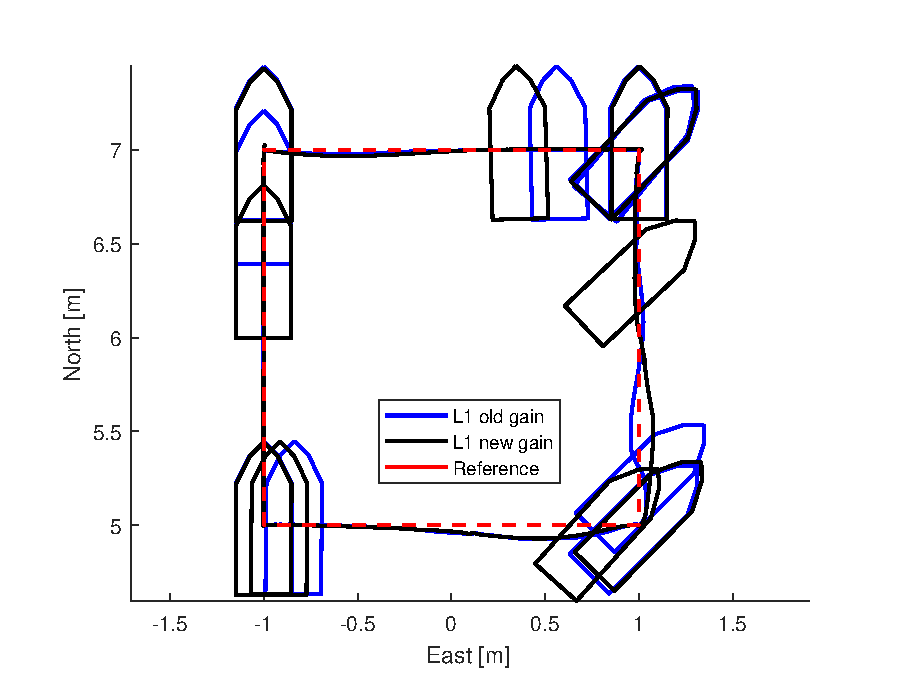
\includegraphics[width=0.9\textwidth]{adjustment_plots/4cornerimprovement.eps}
\caption{4-corner test comparing predictor gain adjustment}
\label{fig:4corner_newL2}
\end{figure}




\begin{table}[h!]
\centering
\caption{Performance metric comparison - Updated L2 gain}\label{table:comparingL2gaintable}
\begin{tabular}{lllll}
\cline{1-4}
\multicolumn{1}{|l|}{\textbf{L2 gain value}} & \multicolumn{1}{l|}{\textbf{IAE}} & \multicolumn{1}{l|}{\textbf{IAEW}} & \multicolumn{1}{l|}{\textbf{IADC}} &  \\ \cline{1-4}
\multicolumn{1}{|l|}{I*2*1.2*2*\pi} & \multicolumn{1}{l|}{76} & \multicolumn{1}{l|}{1231} & \multicolumn{1}{l|}{253} &  \\ \cline{1-4}
\multicolumn{1}{|l|}{I*2*1.2*2*\pi*3} & \multicolumn{1}{l|}{77} & \multicolumn{1}{l|}{722} & \multicolumn{1}{l|}{155} &  \\ \cline{1-4}
 &  &  &  & 
\end{tabular}
\end{table}

As seen in Fig. \ref{fig:4corner_newL2} and \ref{fig:metric_newL2}, there is not really a significant difference in overall pose error for the 4-corner test. However, the updated predictor gain greatly reduces the power consumption by the IAEW metric, and the actuator wear. This can be seen by Fig. \ref{fig:metric_newL2} and in Table \ref{table:comparingL2gaintableb}, where the final values of the metrics are displayed. The IAEW metric is reduced by $41\%$ and the IADC by $38\%$, which is a substantial decrease. This parameter change will be kept into the second lab session.

\begin{figure}[h!]
\centering
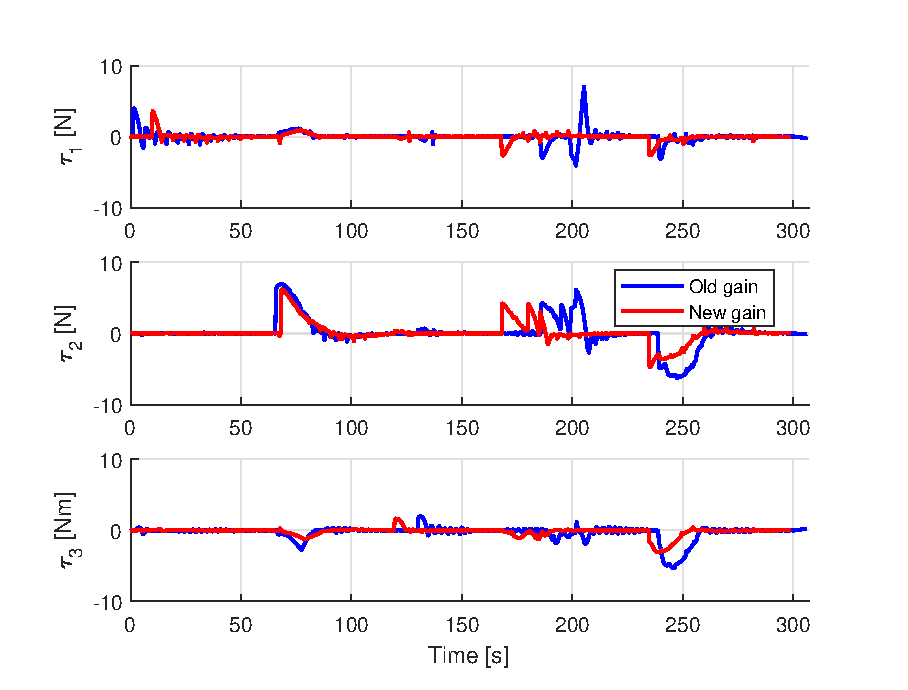
\includegraphics[width=0.9\textwidth]{adjustment_plots/tauimprovement.eps}
\caption{Control inputs comparing predictor gain adjustment}
\label{fig:tau_newL2}
\end{figure}

Fig. \ref{fig:tau_newL2} shows the time evolution of the control input. The overall lower amplitude gives reduced power consumption, but does not lead to a longer run-time of the 4-corner test.

\begin{figure}[!h]
\centering
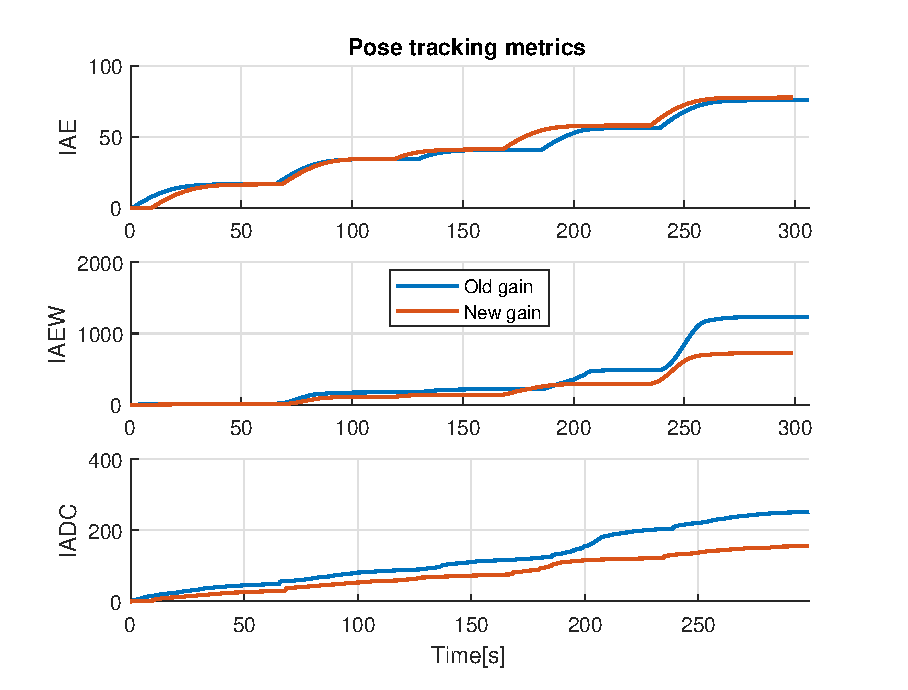
\includegraphics[width=0.9\textwidth]{adjustment_plots/metricimprovement.eps}
\caption{Performance metrics for comparing predictor gain adjustment}
\label{fig:metric_newL2}
\end{figure}